\subsection*{2A.}

\addcontentsline{toc}{subsection}{2A.}

\textbf{Traduce el siguiente modelo Entidad-Relación a su correspondiente Modelo Relacional:}

\begin{figure}[htbp]
    \centering
    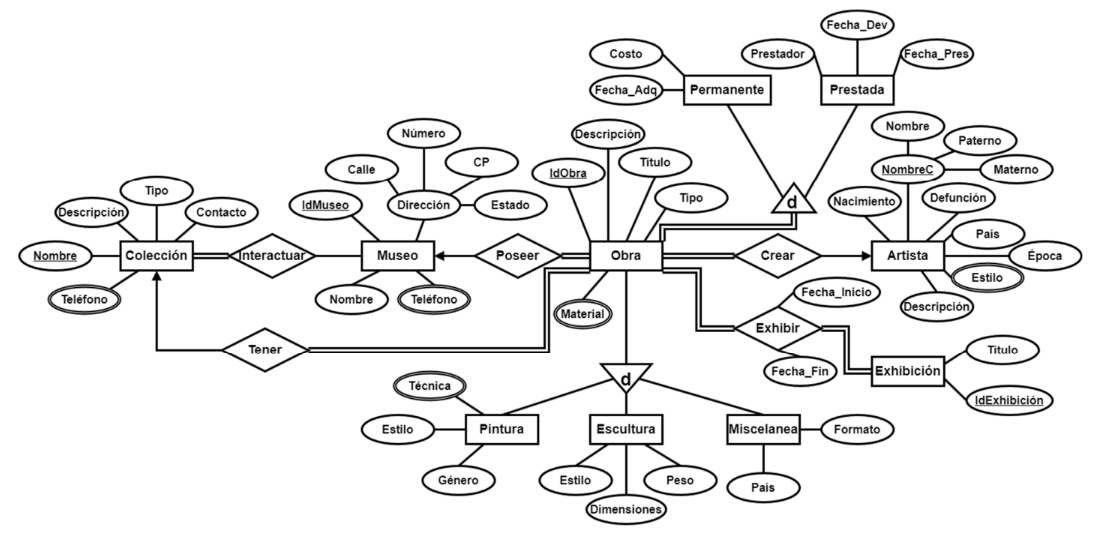
\includegraphics[width=1.1\textwidth]{imagenes/Diagrama(2a)E-R.png}
    \label{fig:mi_imagen}
\end{figure}

\textbf{Entidades fuertes:}\\
\begin{enumerate}
    \item Colección(\underline{NombreColección}, Descripción, Tipo, Contacto)
    \item TeléfonoColección(\underline{Nombre}, \underline{Teléfono})
    \item Museo(\underline{IdMuseo}, Calle, Número, CP, Estado, Nombre)
    \item TelefónoMuseo(\underline{IdMuseo}, \underline{Teléfono})
    \item Exhibición(\underline{IdExhibición}, Título)
    \item Artísta(\underline{Nombre}, \underline{Materno}, \underline{Paterno}, Nacimiento, Defunción, País, Época, Descripción)
    \item Estilo(\underline{Nombre}, \underline{Materno}, \underline{Paterno}, \underline{Estilo})
    \item Obra(\underline{IdObra}, \dotuline{NombreColección}, \dotuline{IdMuseo}, Descripción, Título,Tipo)
    \item MaterialObra(\underline{IdObra}, \underline{Material})
    \item Pintura(\underline{IdObra}, Estilo, Género)
    \item TécnicaPintura(\underline{IdObra}, \underline{Técnica})
    \item Escultura(\underline{IdObra}, Estilo, Dimensiones, Peso)
    \item Miscelanea(\underline{IdObra}, Formato, País)
    \item Permanente(\underline{IdObra}, Fecha-Adq, Costo)
    \item Prestada(\underline{IdObra}, Prestador, Fecha-Dev, Fecha-Pres)
\end{enumerate}
\textbf{Relaciones fuertes}\\
\begin{enumerate}
    \item Interactuar(\dotuline{NombreColección}, \dotuline{IdMuseo})
    \item Exhibir(\dotuline{IdObra}, \dotuline{IdExhibición}, Fecha-inicio, Fecha-Fin)
    \item Crear(\dotuline{IdObra}, \dotuline{Nombre}, \dotuline{Materno}, \dotuline{Paterno})
\end{enumerate}
\textbf{Consideraciones}
\begin{enumerate}
    \item \textbf{Especialización Parcial (Pintura, Escultura, Miscelanea):}\\
    Es parcial y disjunta porque una obra solo puede ser de un tipo a la vez, y además es opcional, ya que pueden existir obras en el catálogo general que no entren estrictamente en ninguna de estas tres categorías. Por esta razón, la tabla Obra conserva todos los datos generales (como \texttt{IdObra}, \texttt{Título}, \texttt{Descripción}) y cada subtabla almacena únicamente los atributos específicos de su categoría.

    \item \textbf{Especialización Total (Permanente y Prestada):}\\
    Es total y disjunta porque toda obra debe ser obligatoriamente permanente o prestada, sin poder e pertenecer a ambas categorías al mismo tiempo. Para evitar duplicar información de forma innecesaria, se mantuvieron las tablas Permanente y Prestada cada una con sus datos correspondientes pero la información general se concentra únicamente en Obra.
\end{enumerate}

\begin{figure}[htbp]
    \centering
    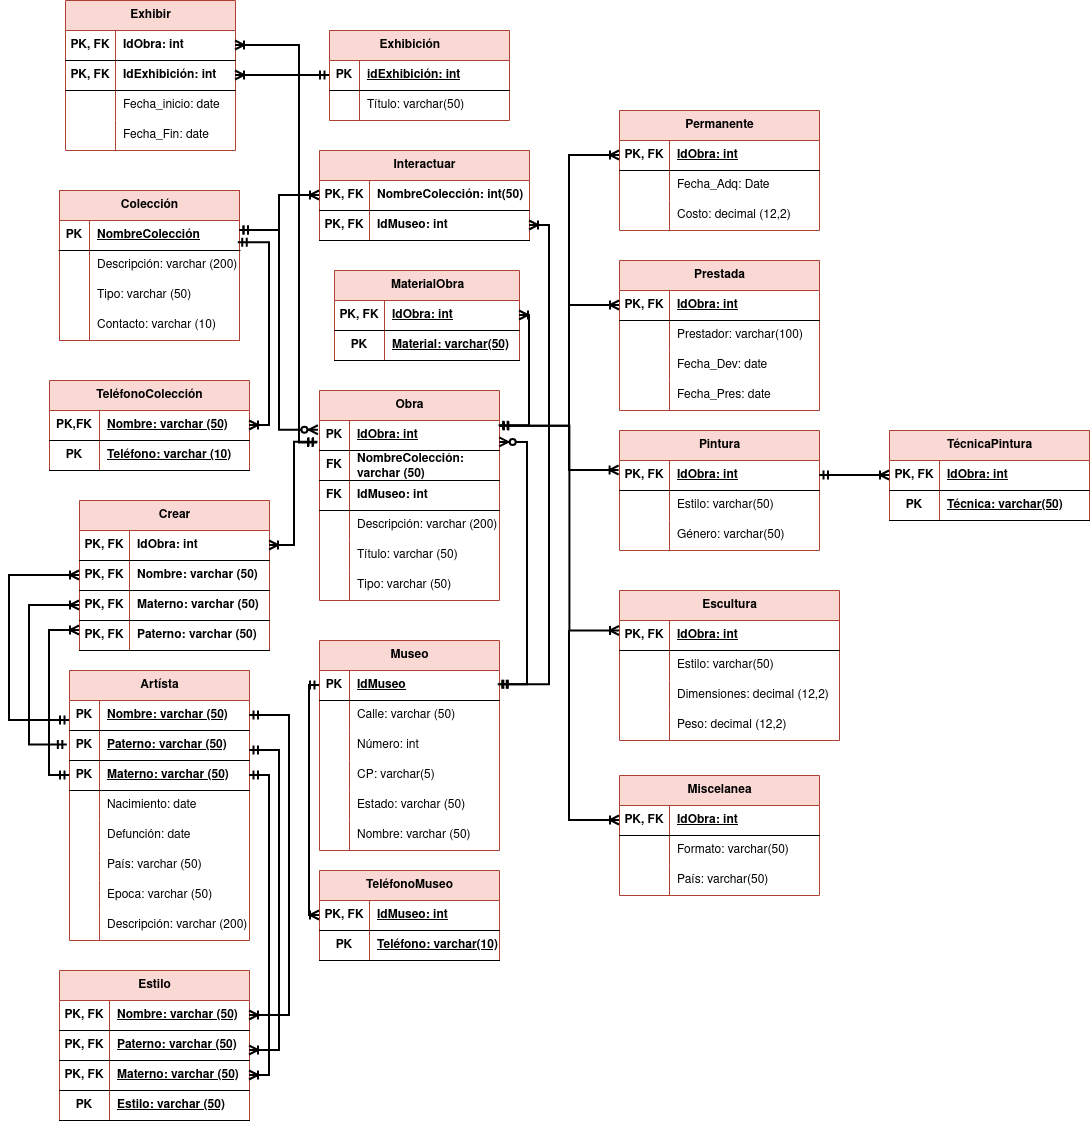
\includegraphics[width=1.1\textwidth]{imagenes/Diagrama2AR.drawio.png}
    \label{fig:mi_imagen}
\end{figure}
